\documentclass[11pt, oneside]{article}   
\usepackage{geometry}                	
\geometry{letterpaper}                   	
\usepackage{graphicx}				
\usepackage{amssymb}

\usepackage{enumitem}

\usepackage{float}
\usepackage{titlesec}

\setcounter{secnumdepth}{4}

\titleformat{\paragraph}
{\normalfont\normalsize\bfseries}{\theparagraph}{1em}{}
\titlespacing*{\paragraph}
{0pt}{3.25ex plus 1ex minus .2ex}{1.5ex plus .2ex}


\usepackage{fancyhdr}
\pagestyle{fancy}
\fancyhead[L]{\today}
\fancyhead[C]{Test Report}
\fancyhead[R]{Group 2: Genzter}


\usepackage{hyperref}
\hypersetup{colorlinks=true,
    linkcolor=blue,
    citecolor=blue,
    filecolor=blue,
    urlcolor=blue,
    unicode=false}

\usepackage[normalem]{ulem}

%SetFonts

%SetFonts


\title{Test Report}
\author{Bengezi, Mohamed\\
		400021279
		\and
		Binu, Amit\\
		400023175
		\and
		Samarasinghe, Sachin\\
		001430998 \\
		\and
		Group 2: Genzter
		}
\date{\today\ }						

\begin{document}
\maketitle
\newpage
\tableofcontents
\listoffigures
\listoftables

\newpage
\section{Revision History}
\begin{table}[h]
\begin{center}
\begin{tabular}{ | c | c | c | c | }
\hline
 \textbf{Date} & \textbf{Version} & \textbf{Description} & \textbf{Author} \\ 
\hline
  01/DEC/17 & 0.0 & Created Test Report & Mohamed Bengezi, Amit Binu, Sachin \\
  &&& Samarasinghe \\
  \hline
  06/DEC/17 & 1.0 & Updated Test Plan, minor fixes & Mohamed Bengezi, Amit Binu \\
\hline 
 & & & \\ 
\hline 
\end{tabular}
\end{center}
\caption{Revision History}
\end{table}

%---------------------
\newpage
\section{Introduction}
\subsection{Summary}
The purpose of this document is to provide a full description of the results of the testing that was outlined and detailed in the Test Plan document. In this document, there is a section detailing the input, expected out, and actual output of all test cases specified in the Test Plan. This testing is for the Timetable Generator Project. 

\subsection{Background}
The Timetable Generator is a mix of a redevelopment of
\href{http://timetablegenerator.io}{this} and \href{https://github.com/ash47/TimetableGenerator}{this}, as well as additions of our own.\\
---------------
\\
The testing has been conducted by the testing team specified in the Test Plan and has been conducted on the team's local machines.\\
---------------
\\
Testing occurred concurrently with the end of the development and implementation phase of the project. This was to ensure that the implementation works as expected, and satisfies all the stated requirements.

\noindent ---------------
\subsection{Test Objectives}
The purpose of the testing of this project is to, as stated above, ensure the presence and integrity of the stated requirements. This includes finding faults and bugs in the program, and remove them as to solidify the system, and make it as robust as possible.

\newpage

\section{Results of Testing}
\subsection{Changes Made}
In regard to the results of the tests detailed in the Test Plan, there were not many changes made to the system because of the testing. There were very minor bugs that were discovered, such as bugs in the UI, as well as a fault in the main scheduling algorithm. The bug was not major enough to disrupt the system in a significant way, but it was there nevertheless.

\subsection{Use of Automated Testing}
Automated testing was used for a large part of the testing phase. We used \href{http://mochajs.org}{Mocha} to test conflict detection, which is when two chosen courses conflict, and there are no alternatives possible. Mocha was also used to test the output of various desired courses. For example, the input might be an Earth Science student's required courses, and Mocha would check if the courses are scheduled in the correct spots.

\subsection{Results of System Tests}
\subsubsection{Test Area 1 \\ Conflict Detection Test}
\begin{enumerate}
\begin{figure}[h]
    \centering
    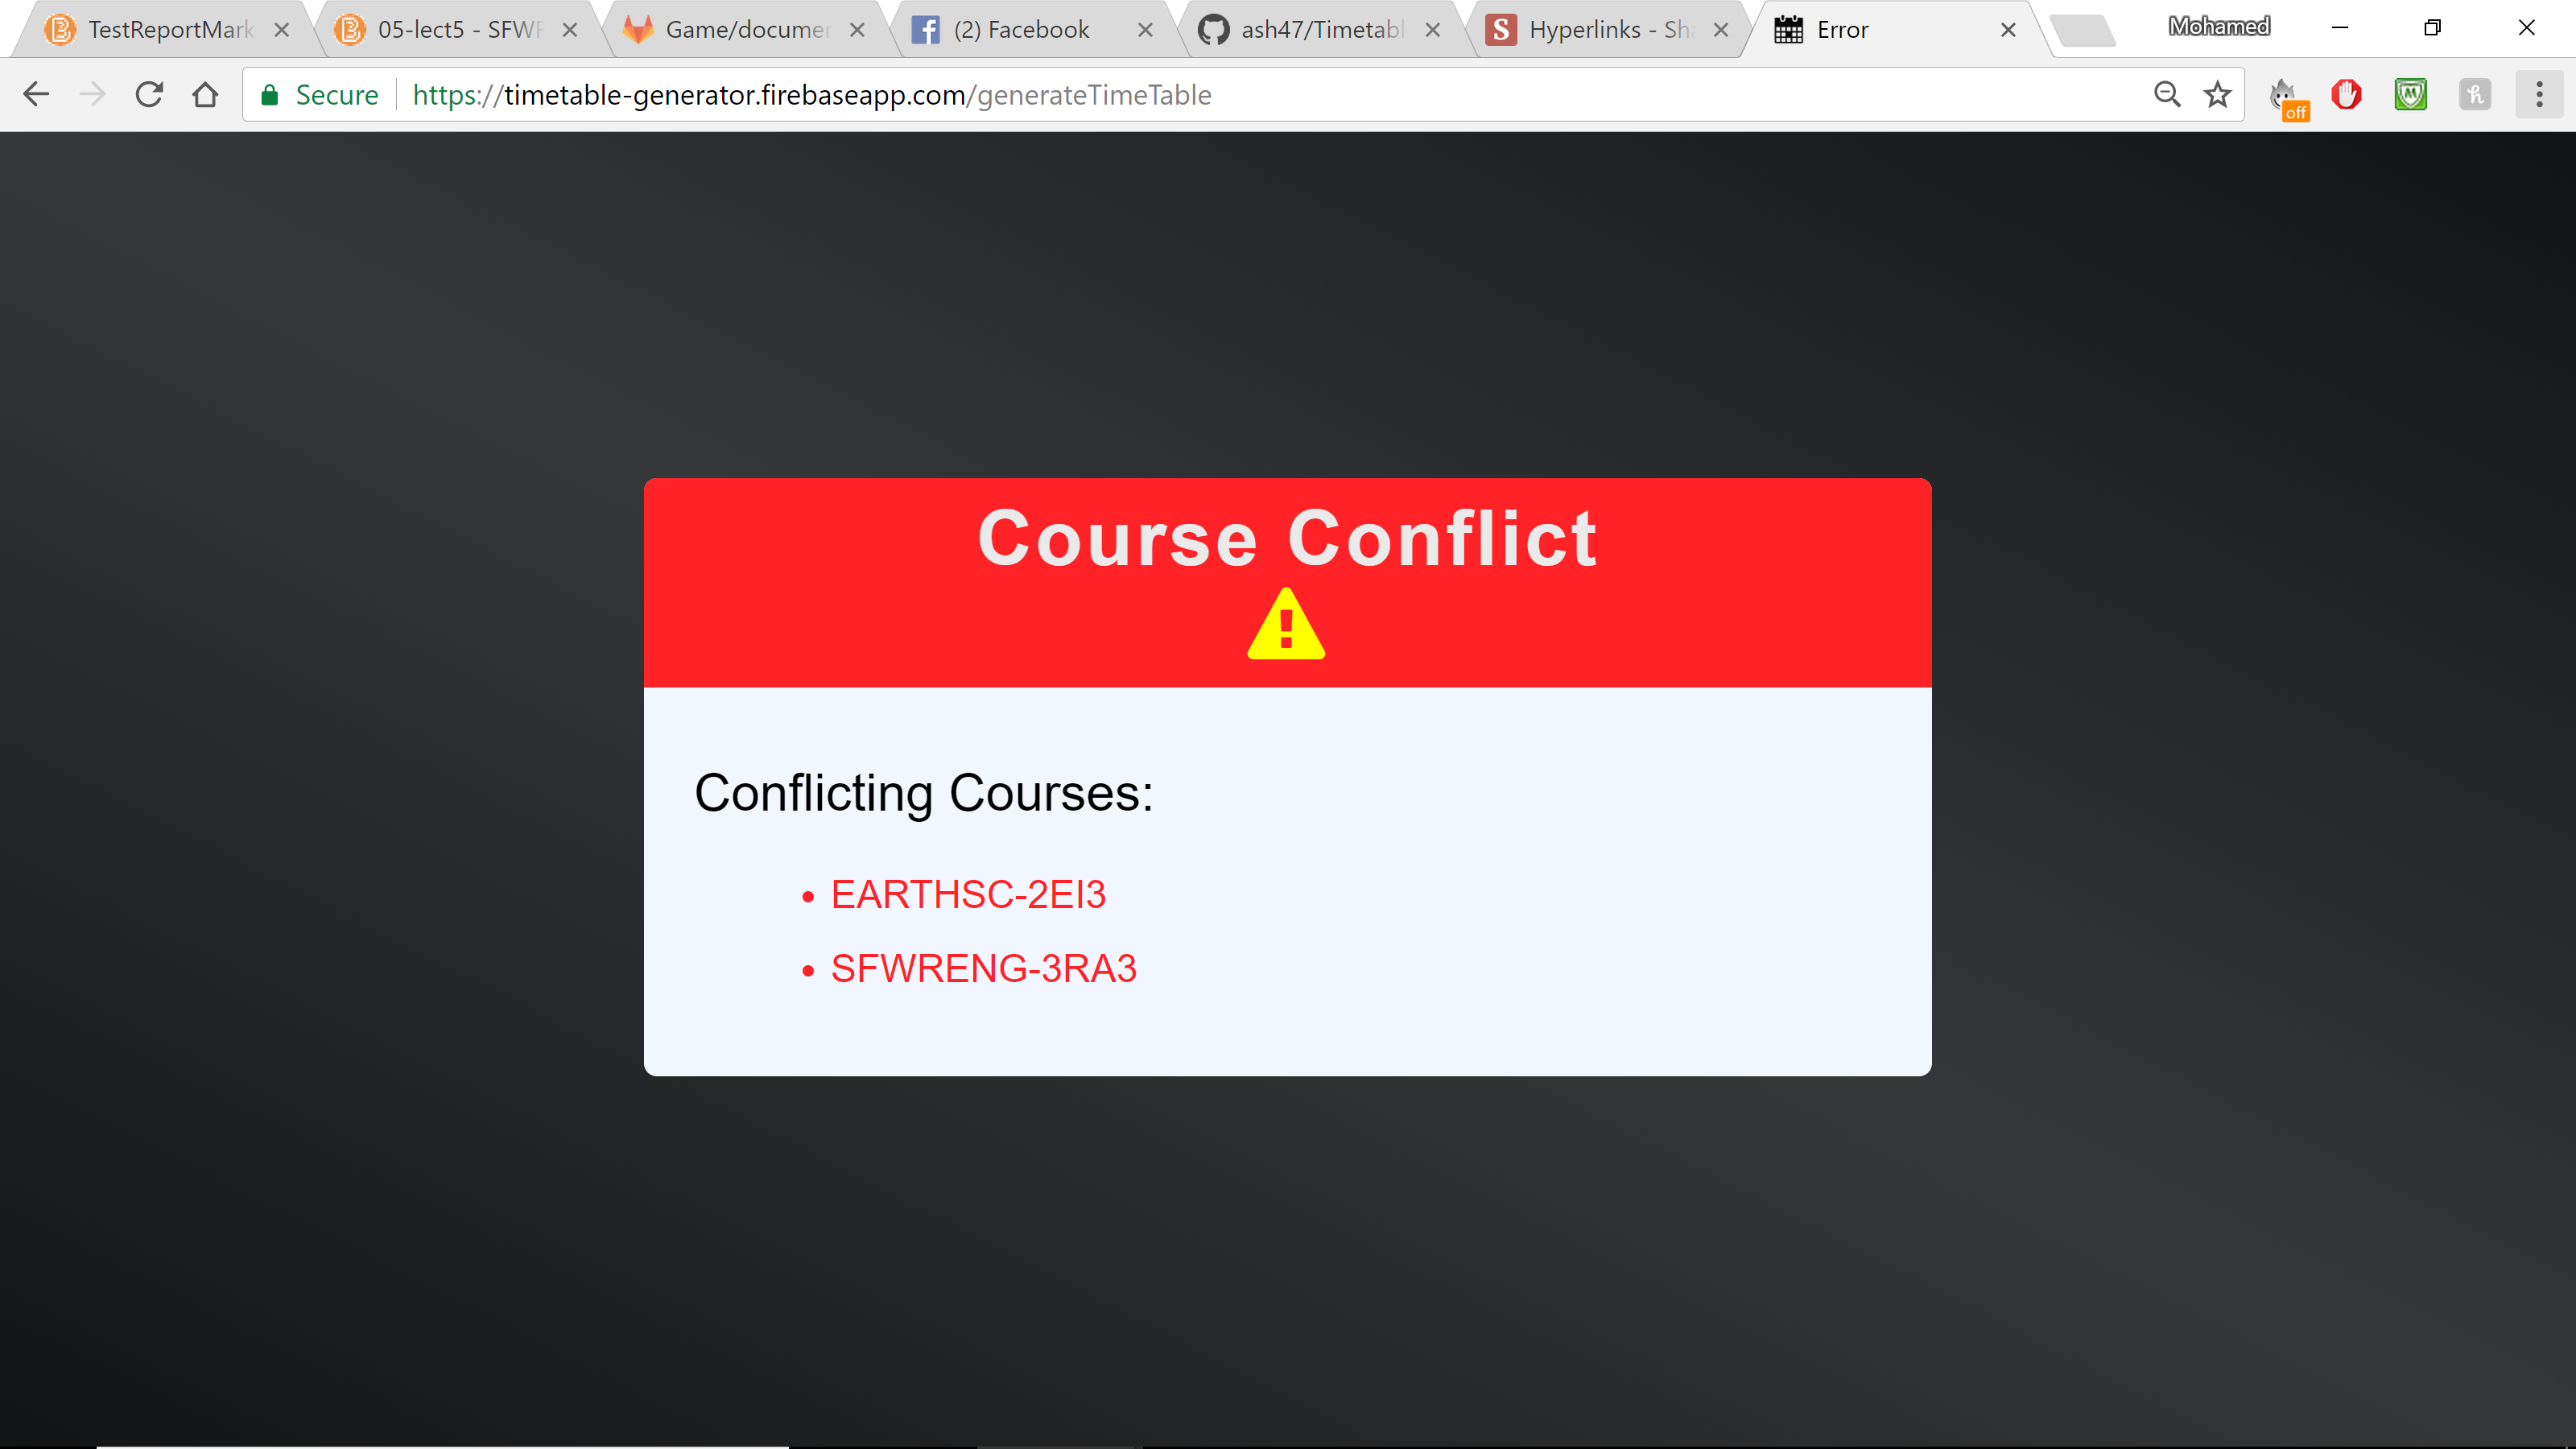
\includegraphics[width=170mm]{Conflict.PNG}
    \caption{Example Conflict Error}
    \label{fig:my_label}
\end{figure}
\item Type: Dynamic \\
Initial State: Homepage \\
Input: SFWRENG 3RA3, EARTHSC 2EI3 \\
Expected Output: Conflict error page \\
Actual Output: Conflict error page \\

\item Type: Dynamic \\
Initial State: Homepage \\
Input: RELIGST-2TA3, SFWRENG 3BB4 \\
Expected Output: Conflict error page \\
Actual Output: Conflict error page \\


\item Type: Dynamic \\
Initial State: Homepage \\
Input: BIOLOGY 2F03, SFWRENG 3MX3 \\
Expected Output: Conflict error page \\
Actual Output: Conflict error page \\


\item Type: Dynamic \\
Initial State: Homepage \\
Input: MATLS 2B03, EARTHSC 2EI3 \\
Expected Output: Conflict error page \\
Actual Output: Conflict error page \\

\begin{figure}[h]
    \centering
    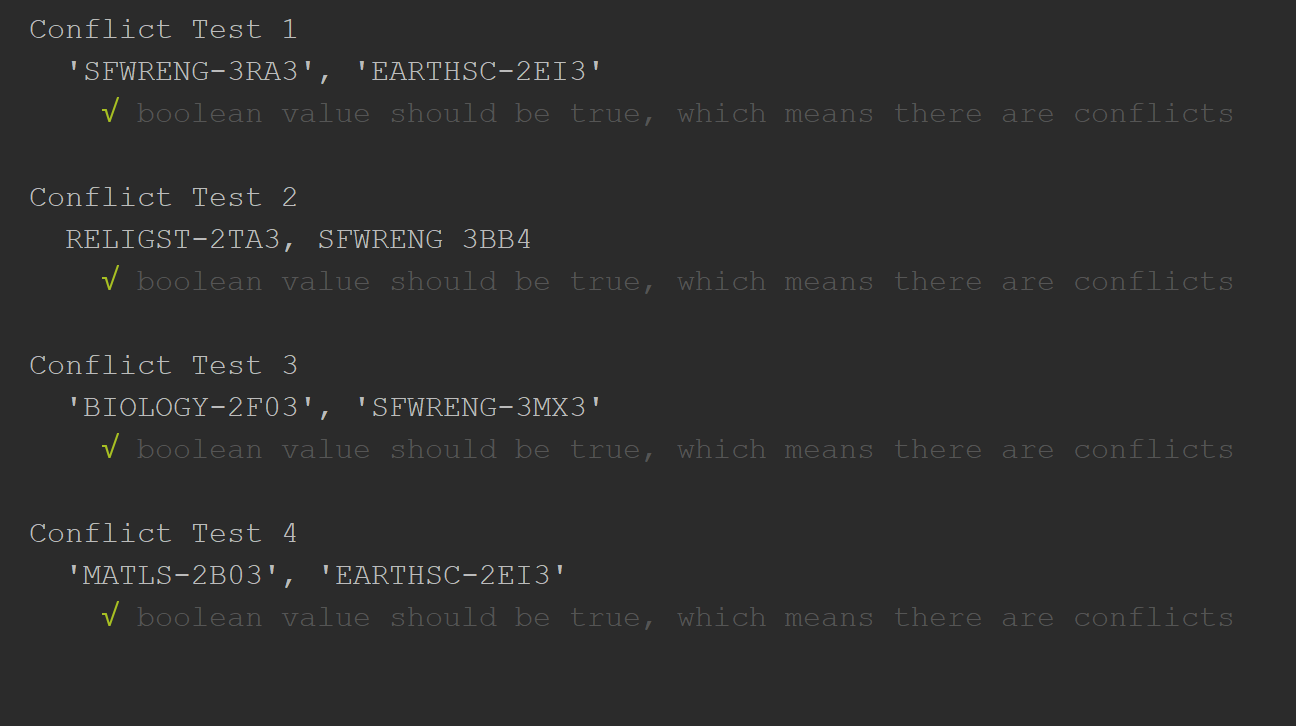
\includegraphics[width=170mm]{CResults.PNG}
    \caption{Conflict Test Results}
    \label{fig:my_label}
\end{figure}
\end{enumerate}



\subsubsection{Test Area 2: Output Timetable}
\begin{figure}[h]
    \centering
    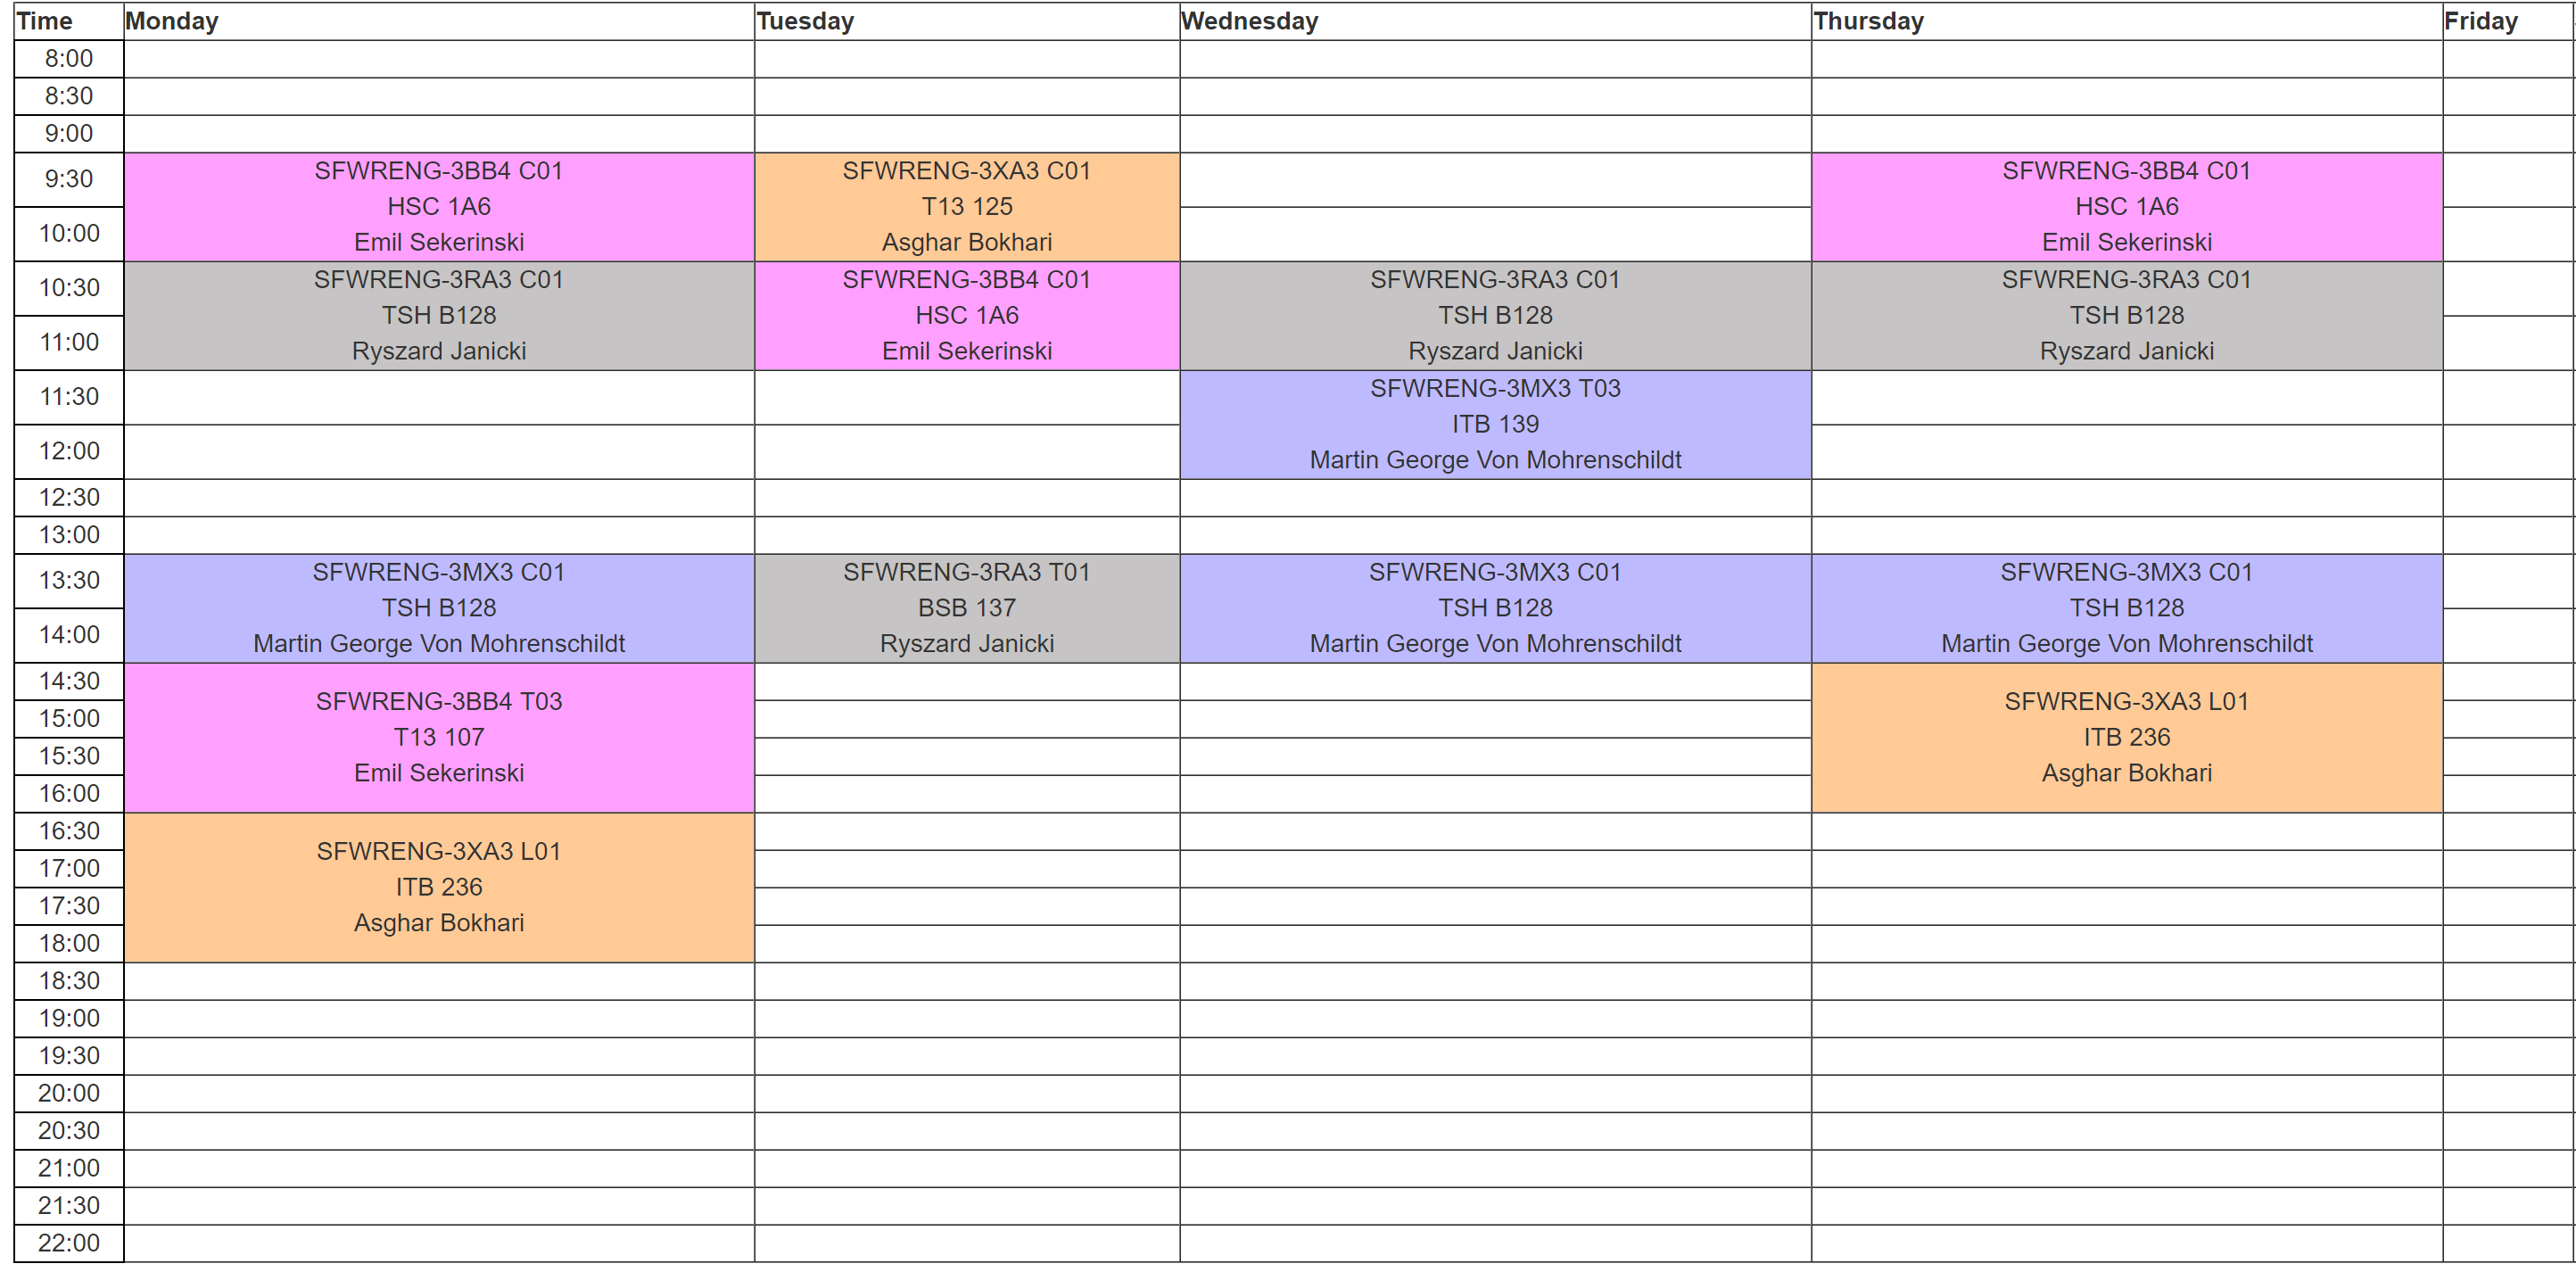
\includegraphics[width=170mm]{Capture.PNG}
    \caption{Example Output}
    \label{fig:my_label}
\end{figure}

\begin{enumerate}
\item Type: Automated \\
Initial State: Homepage \\
Input: SFWRENG 3XA3, SFWRENG 3BB4, SFWRENG 3DB3, SFWRENG 3MX3, COMMERCE 1AA3 \\
Expected Output: Valid Schedule in a timetable format. \\
Actual Output: Color-coded schedule with correct courses and timings \\

\item Type: Automated \\
Initial State: Homepage \\
Input:  ENGINEER-1C03, MATH-1ZC3, MATH-1ZB3,  ECON-1BB3, PHYSICS-1E03, MATLS-1M03 \\
Expected Output: Valid Schedule in a timetable format. \\
Actual Output: Color-coded schedule with correct courses and timings \\

\item Type: Manual \\
Initial State: Homepage \\
Input: RELIGST-2TA3, RELIGST-2QQ3, POLSCI-2I03, POLSCI-4CA3\\
\textcolor{blue}{Expected Output: Valid Schedule in a timetable format.} \\

\item Type: Manual \\
Initial State: Homepage \\
Input:EARTHSC-2EI3, EARTHSC-2C03, GEOG-2UI3, GEOG-2GI3, BIOLOGY-2F03\\
Expected Output: Valid Schedule in a timetable format. \\
Actual Output: Color-coded schedule with correct courses and timings \\

\begin{figure}[h]
    \centering
    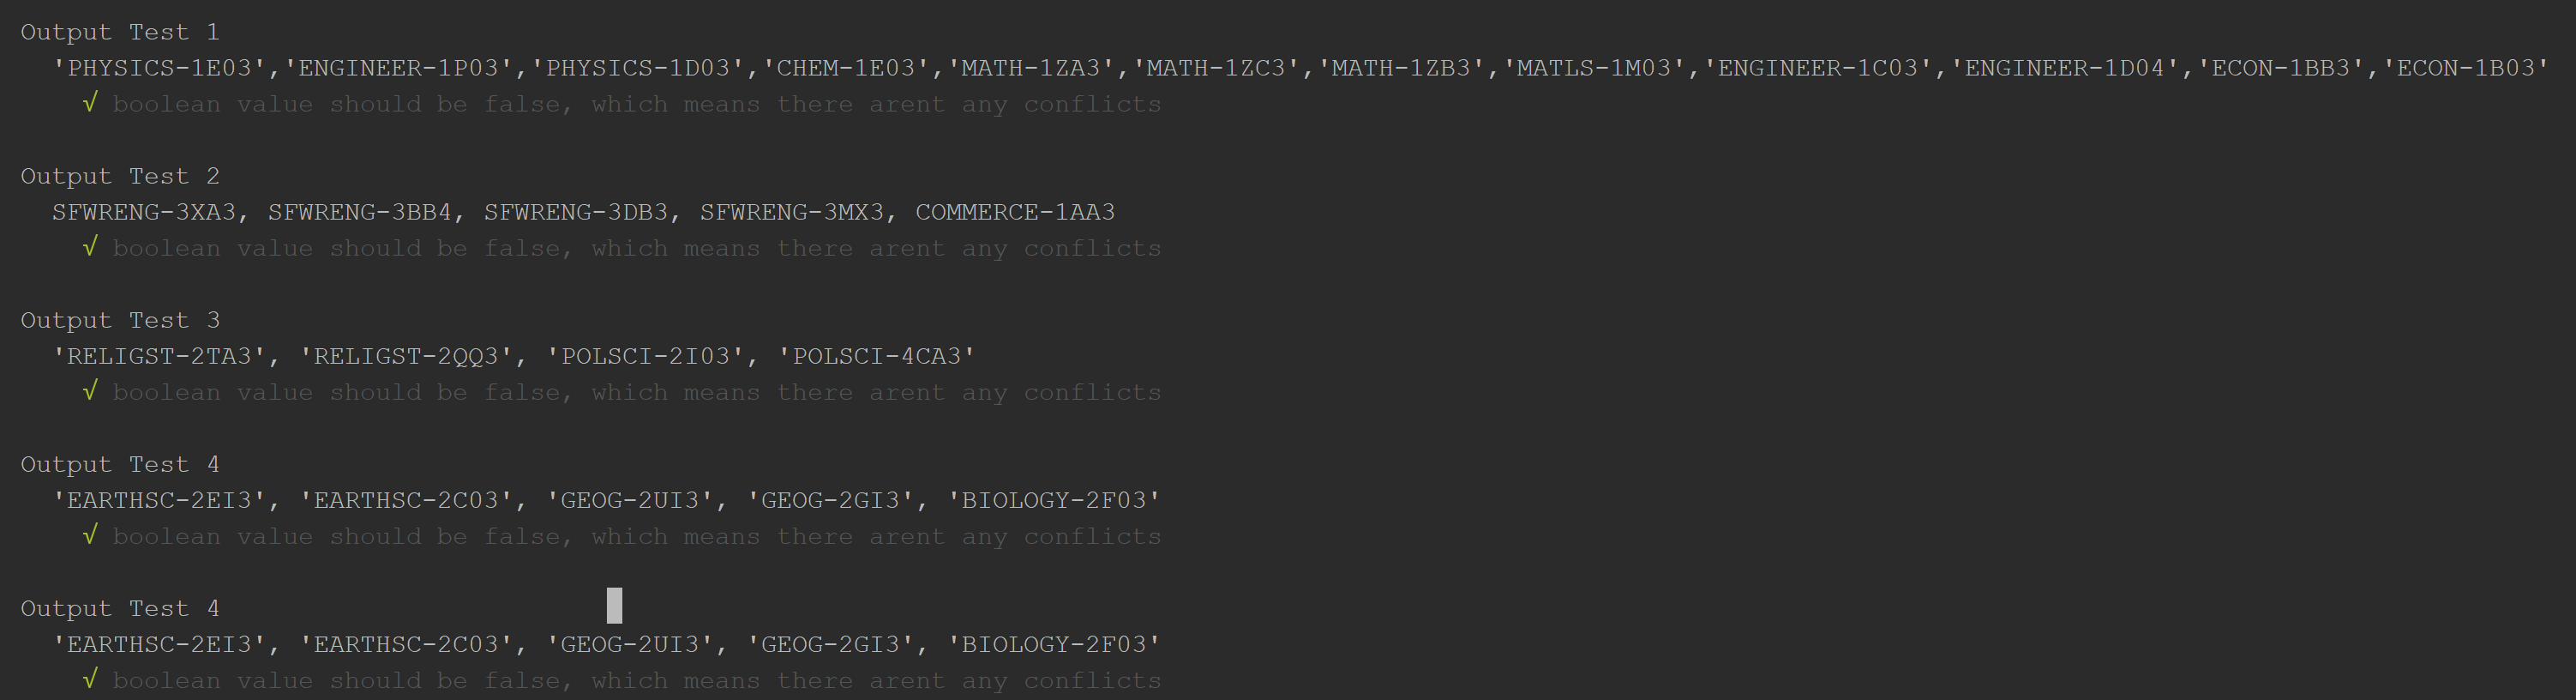
\includegraphics[width=170mm]{OResults.PNG}
    \caption{Output Test Results}
    \label{fig:my_label}
\end{figure} 
\end{enumerate}


\subsubsection{Tests for Non-functional Requirements}
\textbf{Test Area 3: Speed Performance}
\begin{enumerate}

\item Type: Manual \\
Initial State: Homepage \\
Input: SFWRENG 3XA3, SFWRENG 3BB4, SFWRENG 3DB3, SFWRENG 3MX3, COMMERCE 1AA3 \\
Expected Output: Output should be displayed within 3 seconds \\
Actual Output: Schedule was displayed in less than 1 second \\


\item Type: Manual \\
Initial State: Homepage \\
Input:  ENGINEER-1C03, MATH-1ZC3, MATH-1ZB3,  ECON-1BB3, PHYSICS-1E03, MATLS-1M03 \\
Expected Output: Output should be displayed within 3 seconds \\
Actual Output: Schedule was displayed in less than 1 second \\

\end{enumerate}

\subsubsection{Test Area 4: UI}
\begin{enumerate}

\item Type: Manual \\
Initial State: Homepage \\
Input: Any McMaster Course \\
Expected Output: Add course to list of courses \\
Actual Output: Course is added to list \\


\item Type: Manual \\
Initial State: Homepage with list of courses chosen\\
Input:  Pressing the "Remove" button \\
Input: Any McMaster Course \\
Expected Output: Add course to list of courses \\
Actual Output: Course is removed from list \\



\item Type: Manual \\
Initial State: Homepage with list of courses chosen\\
Input:  Pressing the "Generate" button \\
Expected Output: Timetable \\
Actual Output: Timetable \\

\end{enumerate}

\subsubsection{Test Area 5: Maintainability and Robustness}
\begin{enumerate}
\item Type: Static \\
Initial State: Not running \\
Input: Code walk-through and inspection\\
Expected Output: N/A \\
Actual output: The result of this was a cleanup/commenting of the code

\item Type: Dynamic \\
Initial State: Homepage \\
Input: ENGINEER-1C03, MATH-1ZC3, MATH-1ZB3,  ECON-1BB3, PHYSICS-1E03, MATLS-1M03, ECON-1B03, MATH-1ZA3, ENGINEER-1D04, CHEM-1E03\\
Expected Output: Valid Schedule in a timetable format \\
Actual output: The result was a valid, working schedule with all necessary items

\end{enumerate}


\subsubsection{Test Area 6: Browser Compatibility}
\begin{enumerate}
\item Type: Static \\
Initial State: Not running \\
Input: Visit website using different browsers\\
Expected Output: N/A \\
Actual Output: Tested on Chrome, Edge, and Firefox, and responded well to each

\end{enumerate}

\newpage
\section{Traceability}
\begin{table}[h]
\begin{center}
\begin{tabular}{ | c | c | c | c | c | c | }
\hline
 Requirement & TA1 & TA2 & TA3 & TA4 & TA5  \\ 
\hline
 2.7.1 & X & & & &   \\  
\hline
 2.7.2 & & X & X & X & \\
\hline 
 3.2 & & & & X & \\ 
\hline
 3.3 & & & X & & \\
\hline
 3.5 & & & & & X \\
\hline
\end{tabular}
\end{center}
\caption{Traceability Matrix to Requirements}
\end{table}

\begin{table}[H]
\begin{center}
\begin{tabular}{|c|c|}
\hline
Module & Label \\
\hline
Input Parameters Module & M1\\
\hline
Scheduler Module & M2\\
\hline
Output Module & M3\\
\hline
Course Module & M4\\
\hline
\end{tabular}
\end{center}
\label{default}
\caption{Module Labels}
\end{table}


\begin{table}[h]
\begin{center}
\begin{tabular}{ | c | c | c | c | c | c | }
\hline
 Requirement & M1 & M2 & M3 & M4 \\ 
\hline
 2.7.1 & X & & & X \\  
\hline
 2.7.2 & & X & X & X \\
\hline 
 3.2 & X & & X & X\\ 
\hline
 3.3 & & X & X &\\
\hline
 3.5 & X & X & X & X\\
\hline
\end{tabular}
\end{center}
\caption{Traceability Matrix to Modules}
\end{table}
\newpage
\section{Code Coverage Metrics}
In total, we estimate that all the tests conducted covered approximately 75\% of the lines of code contained in the project. \\
\textcolor{blue}{Code Coverage}: Measures the degree to which the source code of a program has been tested. This includes Equivalence testing, Boundary testing, and Control-flow testing.

\subsection{Equivalence Testing}
In the case of the Timetable Generator, the inputs, or courses, are divided into classes such as term 1 courses, term 2 courses, and full semester courses. This is because the generator handles each of these categories separately, so there is a greater chance for bugs and failures. Other classes could be relative to course codes. For example valid course codes, and invalid course codes.
\subsection{Boundary Testing}
Some boundary cases would be using two unit courses as a lower bound/edge, and using a 6 or higher unit course as an upper bound/edge.
\subsection{Control-flow Testing}
Obviously complete control-flow coverage is impossible, but in order to maximize coverage, test cases were used that exercised as many statements, edges, conditions, and paths as possible. It is difficult to fully describe how this was done, seeing as many tests were conducted in addition to the ones listed in this document. Test cases from various McMaster programs' schedule's were used, various different conflict tests were conducted, different amounts of courses were used, and many other tests were used to extend the coverage.
\end{document}  
